\section{25/01/2020 : second model}

\subsection{Decomposed kernels}

It's well known that a symmetric matrix can be decomposed in two vector-sized kernels.
Subsequent convolution with the two (in the case of 2D images) separated kernels
result into the same convolution as the original kernel.
An example is shown in \cite{Sobel}.

In theory it's possible to learn symmetric matrices (or tensors) by separation
in vectors, each for every dimension.

This is going to be the focus of the second model: every 3D convolution is
replaced by three 3D convolutions that have kernel dimension set at 1 except for the
dimension in which the convolution is going to operate.

This way, every ``block'' of convolutions is going to have 30 parameters instead of 246.

The 'stride' subsampling that was characteristic of every convolutional layer
in the first model is being set only at the third layer in each block of
``decomposed'' convolutional layers.

\subsection{Excessive computation of separated convolution layers}

Unfortunately this network, even if it has a lower number of parameters,
its still very computationally expensive.
This is possibly due to the triplication of sweeps on data that has the input 
dimensionality.

To tackle this problem, a subsampling maxpool layer has been added as input layer to
have a preliminary dimensionality reduction.
This follows an observation of genetic algorithm-evolved convolutional neural networks
that were optimized also by running time.
Many of the best-fit genotypes selected by the genetic algorithm
were putting a maxpool layer
on the input with suprising results also in accuracy of the network.

The resulting network has a much reduced amount of trainable parameters: only 1660.

\begin{figure}[h]
\caption{Second model: separated convolutions}
\centering
\includegraphics[width=0.5\textwidth]{second_model.png}
%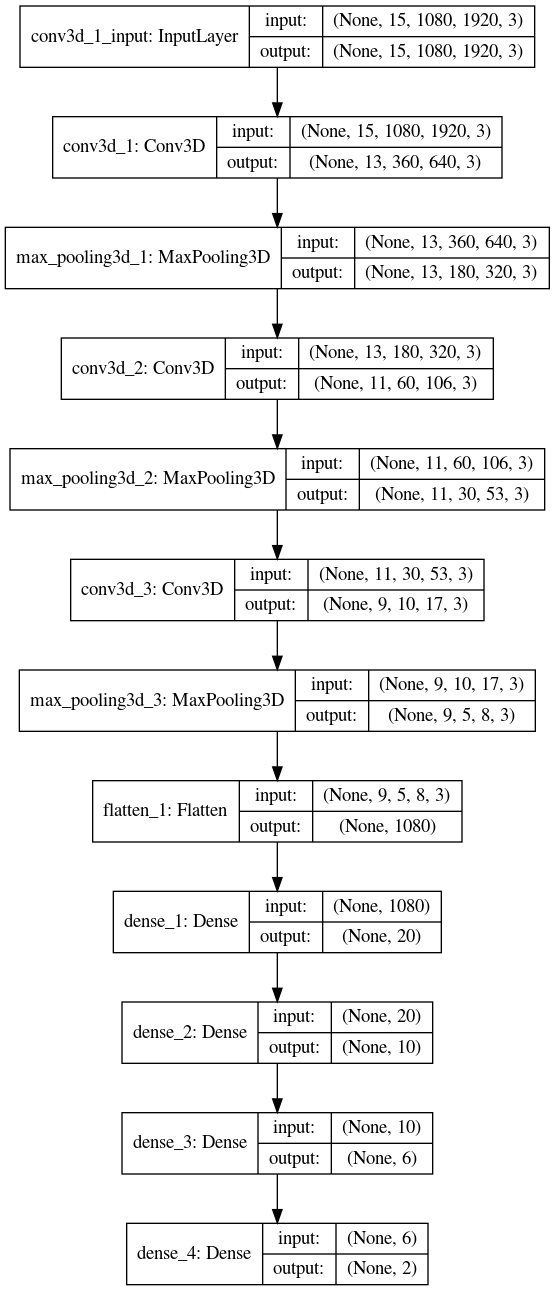
\includegraphics{first_model.png}
\end{figure}

\begin{figure}[h]
\caption{Second model: parameter count for each layer}
\centering
\verbatiminput{second_model_summary.txt}
\end{figure}

\subsection{Excessive loading and pre-processing times}

Moreover, loading a single video in tensor form takes about 7 seconds.
This is not different even using a ramdisk, where all the videos are stored in
memory instead of on the hard drive.

This issue requires a different strategy. Under the current model configuration,
just 15 frames are being used over all 300 frames of each video. Considering the
high loading time of a single video this is quite a waste.
A better approach could be to load and process multiple 15-frames slices after a video
has been loaded.

This will cause a stronger ``learning intensity'' per epoch, as multiple calls to
the fit function will happen for every video.

Memory limits need to be taken into consideration with these changes.
A 15-frames uncompressed slice requires 93.3 MB. A conservative memory allocation
can be 2GB, hence about 20 slices can be loaded from a video.

Such changes come very handy also to tackle the class unbalance problem, which can
be dealt by submitting 5 slices for every fake video and 21 slices for every real
video, which will amount to the previously reported 4.2 ratio of fake videos / real videos.

By submitting 5 slices for every fake video and 21 slices for every real one, one ``new'' 
epoch will have processed 3232. Hence, it would be equivalent as $8.08$ epochs in the 
first model.

To keep a fair comparison with the first model, the amount of videos loaded at every epoch
will be one eight, i.e. 50 videos.

\subsection{Changes in activation functions and optimizing method}

The fully connected layers have been added the $\tanh$ activation function.
The co-domain of the function between -1 and +1 has possibly some advantages.
Vanishing gradient might still be an issue, hence ELU should be considered in the future.

Adam has been used as optimization method, due to using momentum.

\subsection{A note on the platforms used}

\emph{MLFlow} it's a python library employed to track all the experiments, artifact archive,
parameter and metric logging. It provides a convenient user interface to navigate
plots of evolutions of the metrics trough time.

\emph{Floyd Hub} is a remote service that provides easy deployment of runs 
on powerful
hardware such as nodes with NVidia K80 GPUs. It's a rental, so it comes with a price.


\subsection{Second model - an additional larger variant}

As a way to make proper use of the newly-rented GPUs from floydhub,
a larger version of the aforementioned model has been trained.
Among the differences: the number of convolutional blocks has been
increased from 3 to 7. This was made possible by the removal of the strides in the 
ending layer of each convolutional block. This reduced the dimensionality reduction
allowing more convolutional blocks (and max pool layers).
Moreover, the full initial dimensionality has been given to the convolutional blocks by
removing the initial maxpool layer.
Also, the first dense layer has been increased from 20 to 50. 
These changes resulted in a much higher trainable parameter count: $47,075$

\begin{figure}[h]
\caption{Second model: separated convolutions - larger variant}
\centering
\includegraphics[width=0.3\textwidth]{second_model_larger.png}
\end{figure}

\begin{figure}[h]
\caption{Second model - larger variant: parameter count for each layer}
\centering
\scriptsize
\verbatiminput{second_model_larger_summary.txt}
\end{figure}

\subsection{Performances of the second model and the larger variant}

Both models failed again to even hint at the learning some differences between the
two categories, having mean accuracy oscillating around 0.5, basically a coin toss.

\begin{figure}[h]
\caption{Second model: accuracy - vanilla and larger variant}
\centering
\includegraphics[width=1.3\textwidth]{second_model_mean_accuracy.png}
\end{figure}

\subsection{Reflecting on mistakes and future directions}

First of all, in the second model the advice given by \cite{Burlacu}
of \emph{not} using separated convolutions on the first layers was mistakenly not
considered. Moreover, having separated convolutions does not mean reduced computation
by the triplication of the number of sweeps. Especially when the kernel size
is kept as low as 3. It may make more sense if the kernel size would be much higher.

Another huge issue is that $90\%$ of the video is useless for the task of deepfake detection.
It may be more useful to identify a smaller window where the face is located
and concentrate the learning only on that sub-tensor. That would result in faster
learning times,hence more dataset sweeps (epochs) and inferior signal/noise ratio. A library such as \cite{pyface} can be used for the task.

Also, every fit call is currently processing one single datapoint, minibatch learning
needs to be seriously considered to take full advantage of the GPU.

Industry practices suggest using an incresing number of filters as the network gets deeper.
